\documentclass[letterpaper, 11pt]{article}
\usepackage{nopageno} % For removing page numbers
\usepackage[utf8]{inputenc}
\usepackage{color, colortbl} % For table coloring
\usepackage{titling} % For positioning of title preamble
\usepackage[margin=0.75in]{geometry} % For margin width setting
\usepackage{comment} % For block commenting
\usepackage{float} % For table positioning
% For math equation formatting
\usepackage{amsmath, amssymb, amsfonts}
\newcommand{\PMod}[1]{\ (\mathrm{mod}\ #1)}
\newcommand{\Mod}[1]{\ \mathrm{mod}\ #1}
\usepackage{parskip} % For automatic paragraph spacing/formatting
\usepackage{relsize} % For increased math mode font sizing
% For code blocks
\usepackage[dvipsnames,table]{xcolor}
\usepackage[most]{tcolorbox}
\usepackage{lmodern}
\renewcommand{\ttdefault}{lmtt}
\usepackage{listings, minted}
\lstset{
    basicstyle=\ttfamily\footnotesize,
    keepspaces=false,
    showstringspaces=false,
    keywordstyle=\color{blue},
    commentstyle=\sffamily\itshape\color{Green}\scriptsize,
    stringstyle = \color{red},
    breaklines=true,
    breakatwhitespace=false,
    tabsize=2
}
\tcbset{
    colback=gray!5!white,
    colframe=gray!75!black,
    oversize,
}
\setlength{\extrarowheight}{2pt}
\usepackage{titlesec} % Custom styling for section titles
\titleformat{\section}
  {\normalfont\LARGE\bfseries}{\thesection}{1em}{}
\titleformat{\subsection}
  {\normalfont}{\thesection}{1em}{}
% For side-by-side figures
\usepackage{multicol}
\usepackage{makecell}
% For horizontal lists
\usepackage{enumitem, tasks, varwidth}
% For custom page numbers
\usepackage{fancyhdr, lastpage}
\pagestyle{fancy}
\fancyhead{}
\fancyfoot{}
\renewcommand{\headrulewidth}{0pt}
\usepackage[skip=2pt]{caption}
\usepackage{graphicx}
\graphicspath{{../Images/}}

% Move title area to the top of the page
\setlength{\droptitle}{-4em}
\addtolength{\droptitle}{-4pt} 
\renewcommand{\arraystretch}{1.25}
% Disable paragraph indenting
\setlength{\parindent}{0pt}

\usepackage[none]{hyphenat}
\usepackage{times}
\usepackage{soul}

\title{CS430 Homework 7}
\author{Brendan Nguyen}
\date{Due: Sunday, May 7, 2023}

\begin{document}

\maketitle

\section*{Question 1 (80 points)}

Given the relation with the following attributes ACFSBDM.

Note that C is the key. This relation has this set of functional dependencies: FS $\to$ B, A $\to$ D.

\begin{enumerate}[label={\alph*}),leftmargin=*]
    \item Explain why this relation is not in BCNF.

    The relation has dependent elements, B and D, which are dependent on other elements so it cannot be in BCNF.
    
    \item Decompose this relation into BCNF.

    The composition of the relation into BNCF is ACFSM with the relations FSB and AD also existing.
    \begin{figure}[H]
        \centering
        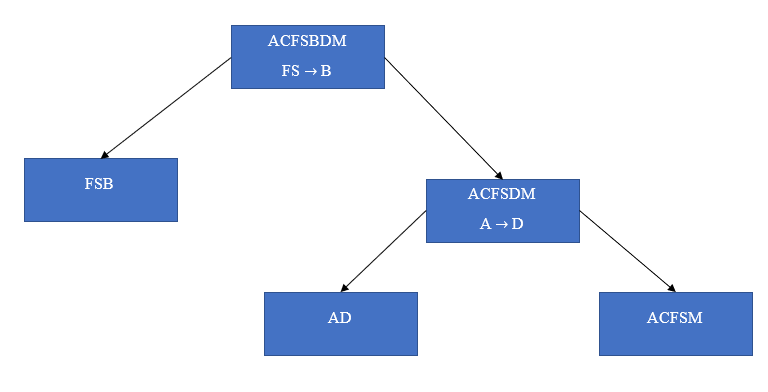
\includegraphics[scale=0.7]{hw7-1b.png}
    \end{figure}
\end{enumerate}

\section*{Question 2 (20 points)}

Write the SQL statements to:
\begin{enumerate}[label={\alph*}),leftmargin=*]
    \item Create user joe with password joe123.

\begin{tcolorbox}
\begin{lstlisting}[language=SQL]
CREATE USER joe IDENTIFIED BY joe123;
\end{lstlisting}
\end{tcolorbox}

    \item Write the SQL statement to give \texttt{SELECT} and \texttt{INSERT} access to user joe to table Sailors. Give access such that user joe can further give access to other users. 

\begin{tcolorbox}
\begin{lstlisting}[language=SQL]
GRANT SELECT, INSERT ON Sailors TO joe WITH GRANT OPTION;
\end{lstlisting}
\end{tcolorbox}
\end{enumerate}


\end{document}
